\documentclass{beamer}

\usepackage[utf8]{inputenc}
\usepackage[T1]{fontenc}
\usepackage[spanish]{babel}
\usepackage{booktabs}
\usepackage{graphicx}
\usepackage{tabularx}
\usepackage{amsmath}

\usetheme{Madrid}
\usecolortheme{default}
\setbeamertemplate{navigation symbols}{}
\setbeameroption{hide notes}
\graphicspath{{../images/}}

\title[Indicadores de Ocupabilidad]{Indicadores de Ocupabilidad de MINCETUR}
\subtitle{14 flujos MapReduce con output real}
\author[Pezo y Pérez]{Sergio Sebastian Pezo Jimenez \and Arbués Enrique Pérez Villegas}
\institute[UNI]{Universidad Nacional de Ingeniería\\CC531 Análisis en Macrodatos}
\date{22 de septiembre de 2026}

\newcommand{\queryslide}[4]{%
\begin{frame}{#1}
\small

\begin{block}{Mapper}
#2
\end{block}

\begin{block}{Reducer}
#3
\end{block}

\begin{alertblock}{Output real}
{\ttfamily\scriptsize #4}
\end{alertblock}
\end{frame}
}

\begin{document}

% ------------------------------------------------
% Portada
% ------------------------------------------------
\begin{frame}
  \titlepage
  \note{Ambos: presentar el objetivo y anunciar que cada query mostrará Mapper, Reducer y output real.}
\end{frame}

% ------------------------------------------------
% Contenido
% ------------------------------------------------
\begin{frame}{Contenido}
  \tableofcontents[hideallsubsections]
  \note{Sergio: presentar brevemente el recorrido de la exposición.}
\end{frame}

% ================================================================
\section{Datos y entorno}
% ================================================================

\begin{frame}{Datos, entorno y recorrido}
\begin{columns}[T,onlytextwidth]

\column{0.47\textwidth}
\textbf{Dataset consolidado}
\begin{itemize}
  \item Periodo 2019--2025-I.
  \item 38\,730 registros.
  \item 24 columnas.
  \item 25 departamentos.
  \item El cambio de esquema fue normalizado.
  \item Se usa TT/TT para evitar doble conteo.
\end{itemize}

\column{0.49\textwidth}
\textbf{Entorno Hadoop 3.5.0}
\begin{itemize}
  \item Docker Compose en un nodo.
  \item HDFS conserva entrada y salidas.
  \item YARN ejecuta los JAR.
  \item La división temporal evita fuga futura.
\end{itemize}

\end{columns}

\vfill
\centering
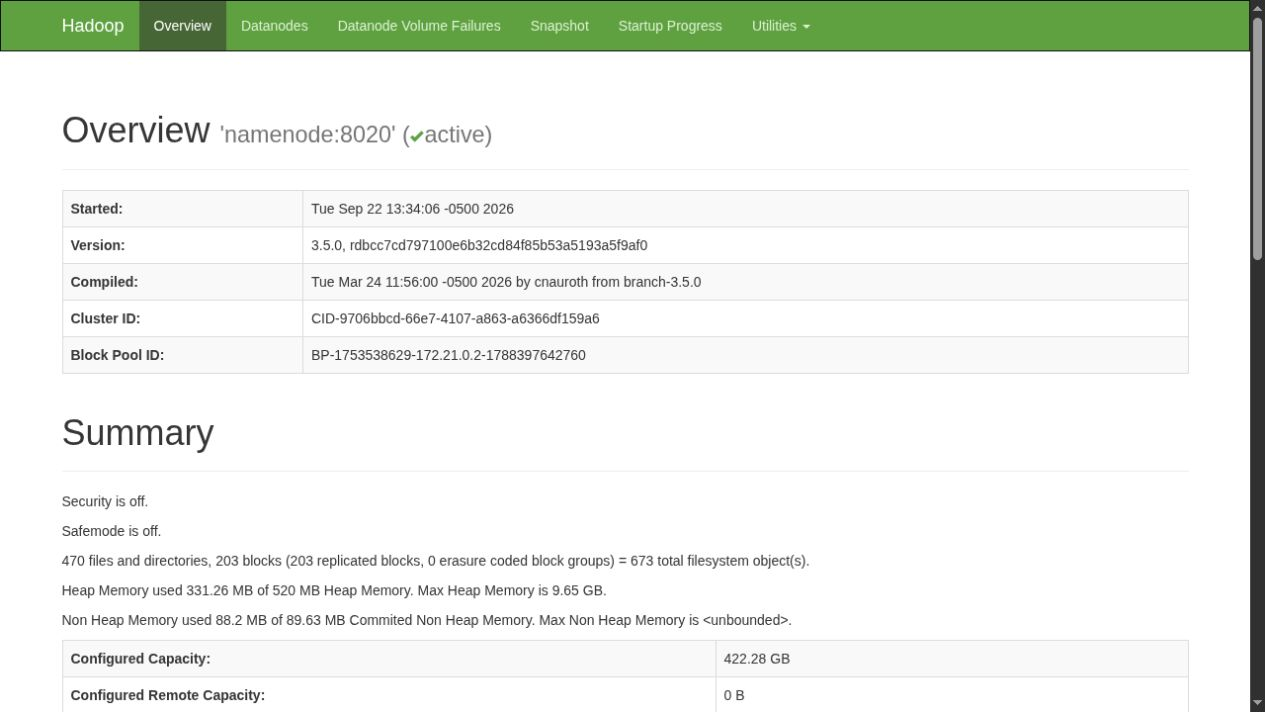
\includegraphics[height=0.13\textheight]{namenode-overview.png}
\hspace{1em}
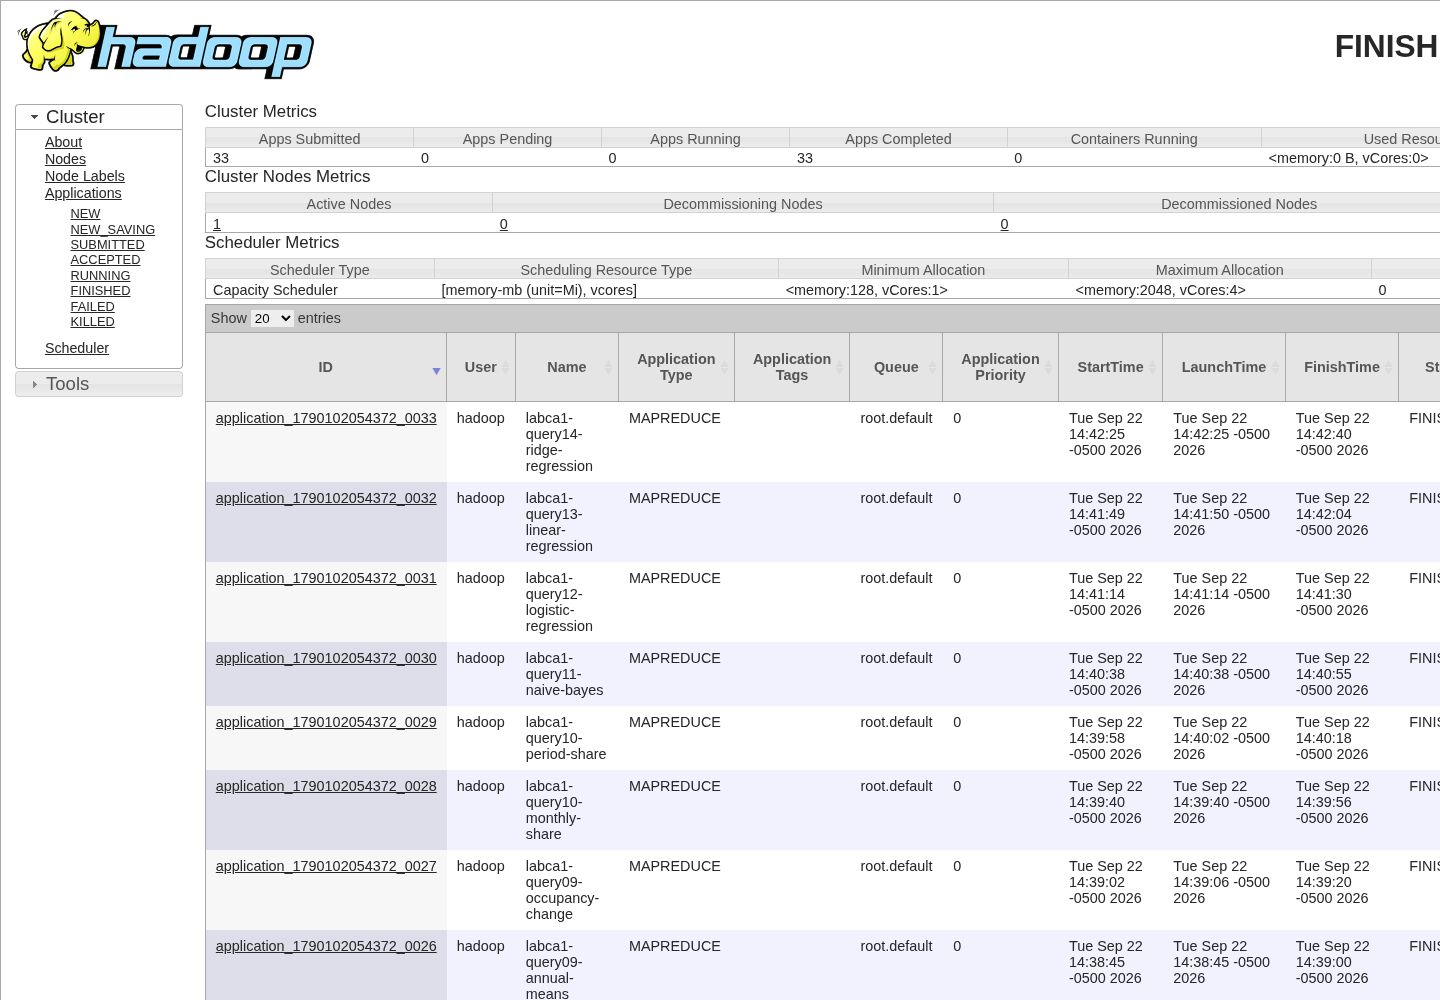
\includegraphics[height=0.13\textheight]{resourcemanager-applications.png}

\note{Arbués: explicar preparación. Sergio: explicar HDFS, YARN y que un nodo valida el flujo, no escalabilidad.}
\end{frame}

% ================================================================
\section{Consultas MapReduce}
% ================================================================

\begin{frame}{Q01 — arribos por origen}
\small
\begin{block}{Mapper}
Emite año como clave y arribos nacionales/extranjeros como valor; filtra TT/TT.
\end{block}

\begin{block}{Reducer}
Suma ambos orígenes para todas las filas del mismo año.
\end{block}

\begin{alertblock}{Output real}
{\ttfamily\scriptsize 2019 national=54897127 foreign=8264767}
\end{alertblock}

\vfill
\textbf{Decisión:} comparar por año revela la caída de 2020 sin mezclar el semestre 2025.

\note{Explicar primero qué emite Map, luego qué agrupa o calcula Reduce y cerrar leyendo el output.}
\end{frame}

\begin{frame}{Q02 — TNOH por departamento}
\small
\begin{block}{Mapper}
Emite año-departamento y el par TNOH,1 para cada fila TT/TT.
\end{block}

\begin{block}{Reducer}
Acumula suma y conteo; calcula la TNOH media por territorio.
\end{block}

\begin{alertblock}{Output real}
{\ttfamily\scriptsize 2024;CALLAO mean\_tnoh=41.5950 | LORETO=12.9917}
\end{alertblock}

\vfill
\textbf{Decisión:} la clave territorial permite comparar departamentos con la misma definición.

\note{Explicar Map, Reduce y luego interpretar el resultado.}
\end{frame}

\begin{frame}{Q03 — TNOH y TNOC por clase}
\small
\begin{block}{Mapper}
Emite año-clase con TNOH, TNOC y contador; usa categoría total y excluye clase TT.
\end{block}

\begin{block}{Reducer}
Promedia ambos indicadores para cada clase de hospedaje.
\end{block}

\begin{alertblock}{Output real}
{\ttfamily\scriptsize 2024;RESORT mean\_tnoh=46.7742 mean\_tnoc=48.2812}
\end{alertblock}

\vfill
\textbf{Decisión:} separar clases muestra patrones que un total nacional ocultaría.
\end{frame}

\begin{frame}{Q04 — empleo por capacidad}
\small
\begin{block}{Mapper}
Emite año-departamento con empleo y habitaciones en filas TT/TT.
\end{block}

\begin{block}{Reducer}
Suma ambos campos y calcula $100 \times empleo / habitaciones$.
\end{block}

\begin{alertblock}{Output real}
{\ttfamily\scriptsize 2024;LIMA employment\_per\_100\_rooms=54.3562}
\end{alertblock}

\vfill
\textbf{Decisión:} la razón normaliza capacidades distintas y hace comparable cada territorio.
\end{frame}

\begin{frame}{Q05 — estacionalidad mensual}
\small
\begin{block}{Mapper}
Emite mes como clave y arribos/pernoctaciones como valores.
\end{block}

\begin{block}{Reducer}
Suma ambos indicadores para todas las observaciones del mismo mes.
\end{block}

\begin{alertblock}{Output real}
{\ttfamily\scriptsize 01 arrivals=33585654 overnight\_stays=43787718}
\end{alertblock}

\vfill
\textbf{Decisión:} agrupar por mes muestra estacionalidad; enero--junio tiene un año adicional.
\end{frame}

% ================================================================
\section{Estadística y comparación}
% ================================================================

\begin{frame}{Q06 — estadística de TNOH}
\small
\begin{block}{Mapper}
Emite todos los valores TNOH TT/TT bajo la clave común \texttt{TNOH}.
\end{block}

\begin{block}{Reducer}
Ordena 1\,950 valores y calcula media, mediana y desviación poblacional.
\end{block}

\begin{alertblock}{Output real}
{\ttfamily\scriptsize count=1950 mean=21.7433 median=21.3400 stddev=7.0679}
\end{alertblock}

\vfill
\textbf{Decisión:} una clave global sirve aquí porque el volumen es pequeño; no escala a cuantiles masivos.
\end{frame}

\begin{frame}{Q07 — búsqueda de subtexto}
\small
\begin{block}{Mapper}
Compara ``hotel'' con clase, categoría y departamento; emite offset y fila coincidente.
\end{block}

\begin{block}{Reducer}
No se utiliza Reducer: cada coincidencia ya constituye el resultado final.
\end{block}

\begin{alertblock}{Output real}
{\ttfamily\scriptsize matches=11525 | 2022;06;HOTEL;1 ESTRELLA;AMAZONAS;...}
\end{alertblock}

\vfill
\textbf{Decisión:} un job map-only evita una etapa de agregación que no aporta valor.
\end{frame}

\begin{frame}{Q08 — extremos de TNOH}
\small
\begin{block}{Mapper}
Emite año y el par departamento,TNOH para filas TT/TT.
\end{block}

\begin{block}{Reducer}
Calcula medias departamentales dentro del año y selecciona mínimo y máximo.
\end{block}

\begin{alertblock}{Output real}
{\ttfamily\scriptsize 2024 min=LORETO:12.9917 max=CALLAO:41.5950}
\end{alertblock}

\vfill
\textbf{Decisión:} resolver medias y extremos juntos evita un segundo job para este dataset.
\end{frame}

\begin{frame}{Q09 — cambio 2019--2024}
\small
\begin{block}{Mapper}
Job 1 emite año-departamento,TNOH; Job 2 reagrupa promedios por departamento.
\end{block}

\begin{block}{Reducer}
Job 1 calcula medias; Job 2 une 2019/2024 y resta puntos porcentuales.
\end{block}

\begin{alertblock}{Output real}
{\ttfamily\scriptsize APURIMAC change\_pp=-18.7325 | UCAYALI=5.0442}
\end{alertblock}

\vfill
\textbf{Decisión:} dos jobs separan agregación y comparación temporal, haciendo verificable cada etapa.
\end{frame}

\begin{frame}{Q10 — participación extranjera}
\small
\begin{block}{Mapper}
Job 1 emite departamento-mes con arribos; Job 2 cambia la clave a departamento-periodo.
\end{block}

\begin{block}{Reducer}
Calcula porcentaje mensual y después su media por periodo analítico.
\end{block}

\begin{alertblock}{Output real}
{\ttfamily\scriptsize CUSCO PRE=63.3747 IMPACT=20.5234 RECOVERY=58.3507}
\end{alertblock}

\vfill
\textbf{Decisión:} los periodos distinguen choque y recuperación; la media no pondera por arribos.
\end{frame}

% ================================================================
\section{Modelos}
% ================================================================

\begin{frame}{Q11 — Gaussian Naive Bayes}
\small
\begin{block}{Mapper}
Emite cada ejemplo TT/TT codificado bajo la clave común \texttt{MODEL}.
\end{block}

\begin{block}{Reducer}
Separa años, fija la mediana, entrena Gaussian NB y calcula métricas.
\end{block}

\begin{alertblock}{Output real}
{\ttfamily\scriptsize TEST\_2024 accuracy=0.703333 recall=0.286885 f1=0.440252}
\end{alertblock}

\vfill
\textbf{Decisión:} se eligió como línea base probabilística; su bajo recall revela la limitación de independencia.
\end{frame}

\begin{frame}{Q12 — regresión logística}
\small
\begin{block}{Mapper}
Emite las mismas variables y partición temporal bajo la clave \texttt{MODEL}.
\end{block}

\begin{block}{Reducer}
Estandariza con entrenamiento, ajusta 200 iteraciones y evalúa probabilidades.
\end{block}

\begin{alertblock}{Output real}
{\ttfamily\scriptsize TEST\_2024 accuracy=0.840000 recall=0.754098 f1=0.793103}
\end{alertblock}

\vfill
\textbf{Decisión:} se eligió por interpretabilidad y mejor equilibrio entre precisión y recall.
\end{frame}

\begin{frame}{Q13 — regresión lineal}
\small
\begin{block}{Mapper}
Emite año, TNOH objetivo y vector de características bajo \texttt{MODEL}.
\end{block}

\begin{block}{Reducer}
Entrena con 2019--2023 y calcula MAE, RMSE y $R^2$ en años posteriores.
\end{block}

\begin{alertblock}{Output real}
{\ttfamily\scriptsize TEST\_2024 mae=3.192221 rmse=4.092002 r\_squared=0.643537}
\end{alertblock}

\vfill
\textbf{Decisión:} da una referencia interpretable para predecir el valor continuo de TNOH.
\end{frame}

\begin{frame}{Q14 — regresión ridge}
\small
\begin{block}{Mapper}
Emite exactamente los mismos ejemplos que Q13 para una comparación justa.
\end{block}

\begin{block}{Reducer}
Ajusta regresión con penalización L2, $\lambda=1$, y calcula las mismas métricas.
\end{block}

\begin{alertblock}{Output real}
{\ttfamily\scriptsize VALIDATION\_2025\_H1 mae=3.013257 rmse=3.879584 r\_squared=0.670320}
\end{alertblock}

\vfill
\textbf{Decisión:} Ridge controla coeficientes correlacionados; la mejora observada es pequeña.
\end{frame}

% ================================================================
\section{Cierre}
% ================================================================

\begin{frame}{Conclusiones y límites}
\begin{columns}[T,onlytextwidth]

\column{0.58\textwidth}
\textbf{Resultados}
\begin{itemize}
  \item Q01--Q05: consultas con múltiples campos.
  \item Q06: estadística descriptiva.
  \item Q07: búsqueda de subtexto.
  \item Q08: extremos agrupados.
  \item Q09--Q10: dos MapReduce enlazados.
  \item Q11--Q12: clasificación.
  \item Q13--Q14: regresión.
  \item Logística: F1 0,7931 en 2024.
  \item Ridge: RMSE 3,8796 en 2025-I.
\end{itemize}

\column{0.38\textwidth}
\begin{alertblock}{Límites}
2025 tiene seis meses.

El clúster usa un nodo.

Algunos promedios no ponderan capacidad.

Los modelos se entrenan en un reducer por el volumen pequeño.
\end{alertblock}

\end{columns}

\note{Ambos: resumir resultados y límites sin afirmar escalabilidad horizontal ni causalidad.}
\end{frame}

% ================================================================
\section{Referencias}
% ================================================================

\begin{frame}[allowframebreaks]{Referencias}
\footnotesize
\begin{thebibliography}{99}

\bibitem{mincetur}
Ministerio de Comercio Exterior y Turismo,
``Indicadores de Ocupabilidad,''
Plataforma Nacional de Datos Abiertos, 2021.

\bibitem{mef}
Ministerio de Economía y Finanzas,
``Ficha Técnica Simplificada para proyectos turísticos,''
2021.

\bibitem{dean}
J. Dean y S. Ghemawat,
``MapReduce: Simplified Data Processing on Large Clusters,''
\textit{Communications of the ACM},
vol. 51, no. 1, pp. 107--113, 2008.

\bibitem{mariani}
M. Mariani y R. Baggio,
``Big data and analytics in hospitality and tourism:
A systematic literature review,''
\textit{International Journal of Contemporary Hospitality Management},
vol. 34, no. 1, pp. 231--278, 2022.

\end{thebibliography}

\vfill
\centering
\Large\textbf{Preguntas y demostración}

\note{Ambos: cerrar y ofrecer ejecutar la query solicitada por el docente.}
\end{frame}

\end{document}
